\subsection{Why virtualized HPC?}
Although HPC workloads are most often run on bare-metal systems, this has started to change 
with the realization that many of the benefits that virtualization offers to enterprises 
can often also add value in HPC environments~\cite{mergen2006virtualization,simons2010virtualizing}. The following are among those benefits:
\begin{itemize}
	\item Supports heterogeneous software stacks
	\item Provides multi-tenancy data security %by isolating user workloads into separate VMs and virtual networks
	\item Offers fault isolation and root access%, and other capabilities not available in traditional HPC environments
	%\item Creates a more dynamic execution environment with live-migrations for load balancing, fault avoidance, etc.
    \item Enables live-migrations for load balancing, fault avoidance, etc.
\end{itemize}

Virtualization can refer to either hypervisor-based full virtualization or container-based OS virtualization. However, container-based virtualization not only lacks support of OS 
heterogeneity, but also falls short in security isolation 
and may incur higher performance interference~\cite{reshetova2014security,sharma2016containers}. Therefore, we will focus on hypervisor-based full virtualization in the remainder of this paper. 

In addition to the above benefits, the performance of virtualized HPC applications has dramatically 
% improved over the past years~\cite{luszczek2011evaluation,younge2011analysis,morabito2015hypervisors}. This is especially true for HPC throughput workloads, which in contrast to Message Passing Interface (MPI) workloads, 
improved over the past years~\cite{luszczek2011evaluation}. This is especially true for HPC throughput workloads, which in contrast to Message Passing Interface (MPI) workloads, 
consist of a large number of independent tasks that can execute in parallel. Throughput workloads represent a 
significant portion of HPC workloads and include financial services, life sciences, electronic design automation, image rendering, etc. In this paper we focus on HPC throughput workloads in the performance evaluation. 
% Studies have demonstrated that the performance gap between virtual and bare-metal for HPC throughput workloads has 
% closed, with just 1 or 2 percentage difference~\cite{michael2018overcommit}. 


\subsection{HPC cloud resource allocation}
If a tenant uses resources intensively, it might make most sense to assign 
a dedicated subset of hardware to the tenant and to appropriately configure VMs on those nodes. 
With two such tenants, one can either place their VMs on a non-overlapping set of nodes (Figure~\ref{fig:allocation1}), 
or place them on the same nodes, being careful to size their VMs to avoid any over-commitment (Figure~\ref{fig:allocation2}). 
The major flaw with these approaches is that resources are statically partitioned and thus susceptible to under-utilization. 
% Although tenants might be very busy during some 
% time periods, they can also be less busy and even idle during other periods. In such cases, sizing VMs as 
% described above can lead to commensurate losses in 
% throughput because the idle resources serving one VM are not available to the other busy VMs.

\begin{figure}
     \centering
     \begin{subfigure}[b]{0.35\textwidth}
         \centering
         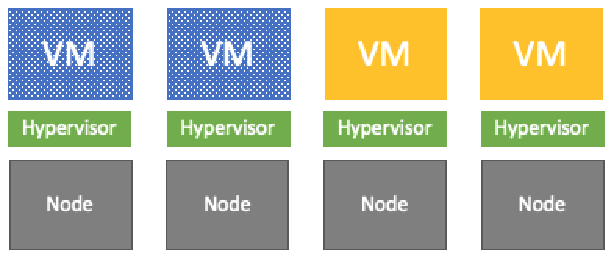
\includegraphics[width=\textwidth]{Figures/allocation1.pdf}
         \caption{Partition on non-overlapping nodes}
         \label{fig:allocation1}
     \end{subfigure}
     \hfill
     \begin{subfigure}[b]{0.35\textwidth}
         \centering
         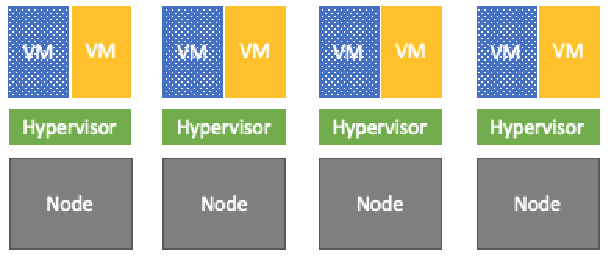
\includegraphics[width=\textwidth]{Figures/allocation2.pdf}
         \caption{Partition on same nodes}
         \label{fig:allocation2}
     \end{subfigure}
     \caption{Example of traditional static allocation. Width of a VM represents
     the fraction of cores assigned to that VM.}
     \label{fig:static_allo}
     \vspace{-0.2in}
\end{figure}



\subsection{Resource over-commitment}
The key to avoiding above resource waste is resource over-commitment. In a 
virtualized environment, resource over-commitment means configuring VMs with more resources than available 
physical ones. For example, on a host with 4 CPU cores and 8 GB memory, one could create two VMs each 
with 4 virtual CPUs and 6 GB virtual memory. 

CPU over-commitment is accommodated by multiplexing virtual 
CPUs onto physical CPUs. In a modern hypervisor like VMware ESXi, a shares-based mechanism can be enabled  
in the scheduler so that VMs with different shares get different portions of the physical CPUs. 
%even in the case of CPU over-commitment. %~\cite{vmware2013scheduler}. 
Furthermore, a work-conserving scheduler 
allows one VM to consume more than its fair CPU shares if there are idle cycles from other VMs. 
Memory over-commitment, on the other hand, is more challenging since multiplexing is not 
applicable. It is achieved by applying a set of memory reclamation techniques, including transparent page sharing (TPS), 
ballooning, compression, and hypervisor swapping~\cite{Waldspurger:2002:MRM:844128.844146,banerjee2013memory}. 
% These techniques differ in the incurred 
% overhead and are individually controlled by the hypervisor based on system memory state.  

Resource over-commitment has been studied in the literature, but previous works either only consider CPU over-commitment, or they do not optimize specifically for HPC workloads~\cite{Tesfatsion2018,shao2011analyzing,gordon2011ginkgo,li2012evaluating}. For example, while~\cite{li2012evaluating} only presents some preliminary memory over-commitment tests using a dummy memory allocation program, \cite{gordon2011ginkgo} adapts memory allocation in a memory over-committed setting by optimizing a 
pre-defined fine-grained performance metric, such as instructions per cycle, which is not commonly available in HPC applications.



